\section{LBM implementation}
The choice of computer language for implementing the LBM methods fell
on \verb!C++!. The main reasons for this choice are that \texttt{C++}
allows both for good possibilities of structuring the good using
object oriented features of the language and good performance. Both of
these are typically highly desired properties of a computer
code. Other alternatives of compiled languages that are known to allow
for high performing code are \texttt{C} or Fortran, but due to the
lack of object orientation in \texttt{C} and the lack of previous
experience in Fortran neither of those were chosen. Both OpenMP and
MPI are also available in \texttt{C++}.

This particular implementation was kept general with respect to
allowing for an extension to three dimensions without having to change
to much of the code. However, due to lack of time, the three
dimensional code was never realised. Sometimes when keeping this
general approach, performance sacrifices had to be made. If the
performance loss was to large, the general approach was put aside and
a 2D specific implementation was used. For a concrete example see
section \ref{sec:hpc:prof}.

One main aim in designing the code interface, was to make it simple to
add new classes, representing e.g. collision operators or boundary
conditions without having to rewrite any existing code. Another was to
make it easy and straightforward to use the code to solve actual
problems. To illustrate how the code may be used in such a case, in
appendix \ref{app:poi_snippet} follows a snippet of how the
implementation is used to model Poiseuille flow.

The performance of the implementation was tested for the different
implementations but is here only presented for the Navier-Stokes case,
section \ref{sec:lbm:ns}, for which it exist comparative work for
reference. A common measure in the case of lattice-Boltzmann
performance analysis is million lattice updates per second (MLUPS). A
crucial parameter in these tests is the lattice dimension, whether the
whole $f$ array fits in the last level cache or not may affect the
results drastically. The results for a single thread execution and for
different grid sizes are presented in fig. \ref{fig:hpc:mlups}. Here
we see a sudden drop about when the grid size passes the cache
size. For large enough grids the update frequency seems to converge to
about 4.5 MLUPS. In most physical systems the $f$ array will not fit
in the cache and if any number should be presented for the performance
of the code, this is it.

The update frequency is a very hardware independent measure, it is
therefore difficult to compare implementations directly unless you
find a benchmark using the exact same hardware setup as you
use. However, there are some tests carried out and even if the numbers
are not to be compared exactly, it may give a good hunch about the
performance of the implementation. In \cite{palabos}, LBM
implementations in different computer languages are compared, the C++
implementation is measured to 3.15 MLUPS. Other results are 4.46 MLUPS
\cite{lbm_bench_thomas}, $1.0-4.6$ MLUPS \cite{lbm_bench_mattila} and
6.18 MLUPS (D3Q19) \cite{lbm_bench_bailey}. The numbers here are of
comparable magnitude with the one in this work of 4.5 MLUPS.

\begin{figure}
\begin{center}
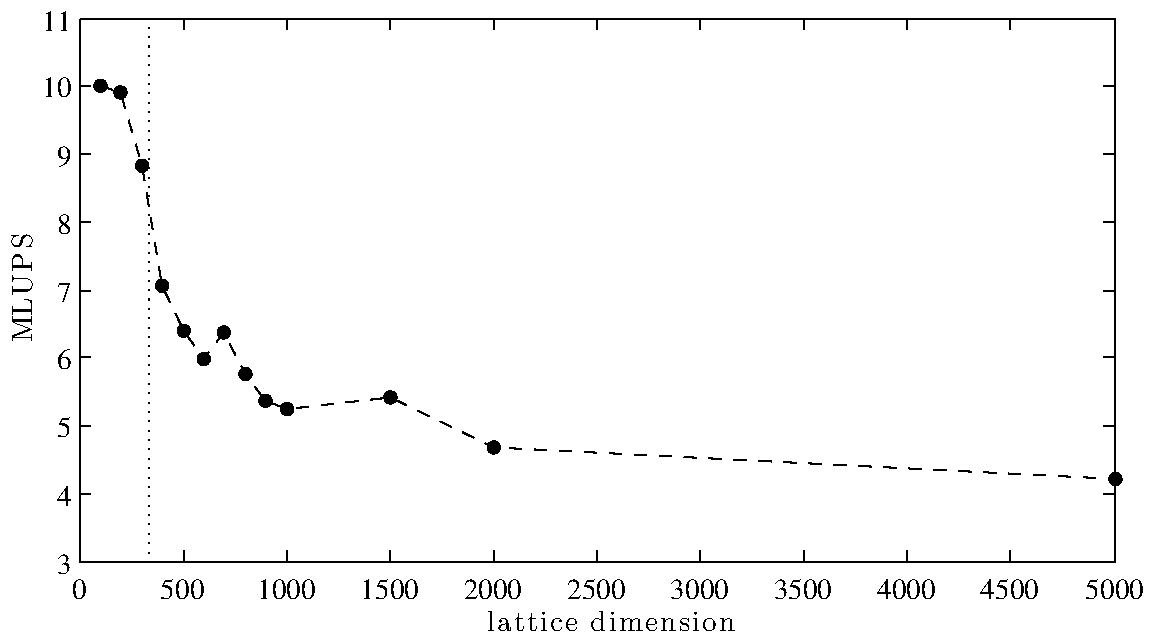
\includegraphics[width=0.9\textwidth]{fig/mlups.pdf}
\end{center}
\caption[Performance of code for different grid sizes.]{Performance of
  code measured in MLUPS (Million Lattice Updates Per Second) for
  different grid sized. The dotted vertical line denotes the grid size
  where the $f$ array has the same size as the L3 cache. These
  computations were carried out on a \texttt{Intel(R) Core(TM) i7-3770
    CPU @ 3.40GHz}.}
\label{fig:hpc:mlups}
\end{figure}

%compiler optimisation 00/1/2/3

\nomenclature{MLUPS}{Million Lattice Updates Per Second}
